\documentclass[12pt]{article}

\title{On numerical anisotropic Newtonian gravitation}
\author{S. Halayka\footnote{sjhalayka@gmail.com}}
\date{\today\;\currenttime}

\usepackage{datetime}
\usepackage{listings}
\usepackage{cite}
\usepackage{xcolor}
\usepackage{graphicx}
\usepackage{setspace}
\usepackage{amsmath}
\usepackage{url}
\usepackage[margin=0.75in]{geometry}
\usepackage{listings}


\usepackage{xcolor}
\lstset { %
    language=C++,
    backgroundcolor=\color{black!5}, % set backgroundcolor
    basicstyle=\footnotesize,% basic font setting
    showstringspaces=false,
}


%\doublespace

%\usepackage[]{lineno}
%\linenumbers


\begin{document}



 
\maketitle

\begin{abstract}
This paper contains a short introduction to anisotropic Newtonian gravitation.
\end{abstract}



\section{Introduction}

First see \cite{halayka} for a short tutorial for C++ programmers on isotropic Newtonian gravitation.
In \cite{halayka} we build an isotropic gravitational field through the use of pseudorandomly generated field lines.

Here we introduce a method for generating anisotropic gravitational fields through the use of spherical linear interpolation.
In effect, we are squishing the gravitational field.
See Figs. 1 - 3.
Anisotropic gravitational fields provide extra acceleration, which is useful for modeling the flat rotation curves in galactic dynamics.
See Figs. 4 and 5.




\section{Brute force: field line intersection density gradient}

Regarding the holographic principle \cite{hooft, susskind}, the number of gravitational field lines for a black hole is related to the event horizon area $A$:
\begin{equation}
n = \frac{A k c^3}{ 4 G \hbar \log 2}.
\end{equation}
For a Schwarzschild black hole in particular \cite{misner}, the event horizon radius $r_s$ is
\begin{equation}
r_s = \sqrt{\frac{A}{4 \pi}} = \sqrt{\frac{n G \hbar \log 2}{k c^3 \pi}},
\end{equation}
and the mass of the Schwarzschild black hole is
\begin{equation}
M = \frac{c^2 r_s}{2 G} = \sqrt{\frac{n c \hbar \log 2}{4 G k \pi}}.
\end{equation}

Where the $\beta$ function is the integer field line collision count, $R$ is the distance from the black hole centre, and $\epsilon$ is some small number:
\begin{equation}
\alpha = \frac{\beta(R + \epsilon) - \beta(R)}{\epsilon}.
\end{equation}
The gradient strength, where $r$ is the receiver radius, is:
\begin{equation}
g = \frac{-\alpha}{r^2}. 
\end{equation}


Below is a small bunch of code to define the $\beta$ function using C++.

The full code can be found at 

\url{https://github.com/sjhalayka/numerical_newtonian_gravity}


\begin{lstlisting}
// Pseudorandom unit vector using Mersenne Twister
vector_3 random_unit_vector(void)
{
	const double z = dis(generator) * 2.0 - 1.0;
	const double a = dis(generator) * 2.0 * pi;

	const double r = sqrt(1.0f - z * z);
	const double x = r * cos(a);
	const double y = r * sin(a);

	return vector_3(x, y, z).normalize();
}

// Spherical linear interpolation
vector_3 slerp(vector_3 s0, vector_3 s1, const double t)
{
	vector_3 s0_norm = s0;
	s0_norm.normalize();

	vector_3 s1_norm = s1;
	s1_norm.normalize();

	const double cos_angle = s0_norm.dot(s1_norm);
	const double angle = acos(cos_angle);

	const double p0_factor = sin((1 - t) * angle) / sin(angle);
	const double p1_factor = sin(t * angle) / sin(angle);

	return s0 * p0_factor + s1 * p1_factor;
}

// Ray-circle intersection function
bool circle_intersect(
	const vector_3 normal,
	const double circle_location,
	const double circle_radius)
{
	vector_3 outline_dir(
		circle_location, 
		circle_radius, 
		0);

	outline_dir.normalize();

	static const vector_3 v(1, 0, 0);

	const double d = outline_dir.dot(v);

	if (d <= 0)
		return false;

	const double d_ = normal.dot(v);

	if (d_ <= d)
		return false;

	return true;
}
\end{lstlisting}

\begin{lstlisting}
// beta function
long long signed int get_intersecting_line_count_integer(
	const long long signed int n,
	const vector_3 sphere_location,
	const double sphere_radius,
	const double D)
{
	const double disk_like = 3.0 - D;

	long long signed int count = 0;

	generator.seed(static_cast<unsigned>(0));

	for (long long signed int j = 0; j < n; j++)
	{
		const vector_3 p = random_unit_vector();

		vector_3 p_disk = p;
		p_disk.y = 0;
		p_disk.normalize();

		const vector_3 normal = slerp(p, p_disk, disk_like);

		if (circle_intersect(normal, sphere_location.x, sphere_radius))
			count++;
	}

	return count;
}
\end{lstlisting}

The Newtonian gravitational variables are acceleration:
\begin{equation}
a_N = \frac{G M}{R^2} = \sqrt{\frac{n G c \hbar \log 2}{4 k \pi R^4}},
\end{equation}
circular orbit speed:
\begin{equation}
v_N = \sqrt{a_N R},
\end{equation}
and gradient strength:
\begin{equation}
g_N = \frac{a_N k 2 \pi M}{R c \hbar \log 2}. 
\end{equation}

The flat rotation curve variables are:
\begin{equation}
v_{\textrm{flat}} = x v_N,
\end{equation}
where $x = 2$ for example.
\begin{equation}
a_{\textrm{flat}} = \frac{v_{\textrm{flat}}^2}{R} = \frac{g R c \hbar \log 2}{k 2 \pi M}.
\end{equation}

Since
\begin{equation}
a_{\textrm{flat}} \propto g
\end{equation}
and
\begin{equation}
a_{\textrm{ratio}} = \frac{a_{\textrm{flat}}}{a_N},
\end{equation}
\begin{equation}
g_{\textrm{ratio}} = \frac{g}{g_N},
\end{equation}
to then find $D$, look for where $g_{\textrm{ratio}} \geq a_{\textrm{ratio}}$, starting from $D = 3$, marching toward $D = 2$.
The Galaxy becomes more and more disk-like as distance from the core increases.

For instance, for the Galactic orbit of the Solar System at $R = $ 3e20 metres, where the mass is $M = $ 1e41 kilograms, and the circular orbit speed is $v = 220000$ metres per second, the ratio is only $2.17551$:
\begin{lstlisting}
#include <cmath>
#include <iostream>
using namespace std;

const double pi = 4.0 * atan(1.0);
const double G = 6.67430e-11;
const double c = 299792458;
const double c2 = c * c;
const double c3 = c * c * c;
const double c4 = c * c * c * c;

const double h = 6.62607015e-34;
const double hbar = h / (2.0 * pi);

const double k = 1.380649e-23;

int main(void)
{
	double M = 1e41;
	double R = 3e20;

	double a_Newton = G * M / (R * R);

	double v_flat = 220000;
	double a_flat = (v_flat * v_flat) / R;

	// ... 2.17551
	cout << a_flat / a_Newton << endl;

	double emitter_radius = 2 * G * M / c2;

	const double emitter_area =
		4.0 * pi * emitter_radius * emitter_radius;

	// Field line count
	// re: holographic principle:
	const double n =
		(k * c3 * emitter_area)
		/ (log(2.0) * 4.0 * G * hbar);

	// ... 5.28417e75
	cout << n << endl;

	return 0;
}
\end{lstlisting}
Of course, solving for the Galactic flat rotation curve using brute force is not feasible due to current processor speed limitations.
Work on an analytical method is underway.


\section{Appendix I -- 1-D Filaments}
Where $D = [1, 3]$:
\begin{lstlisting}
long long signed int get_intersecting_line_count_integer(
	const long long signed int n,
	const vector_3 sphere_location,
	const double sphere_radius,
	const double D)
{
	const double filament_like = (3.0 - D) * 0.5;
	long long signed int count = 0;

	generator.seed(static_cast<unsigned>(0));

	for (long long signed int j = 0; j < n; j++)
	{
		const vector_3 p = random_unit_vector();

		vector_3 p_bidirectional = p;
		p_bidirectional.y = p_bidirectional.z = 0;
		p_bidirectional.normalize();

		const vector_3 normal = slerp(p, p_bidirectional, filament_like);

		if (circle_intersect(normal, sphere_location.x, sphere_radius))
			count++;
	}

	return count;
}
\end{lstlisting}
This method directly goes from spherical to filament-like.
There is another, indirect method, in which one first becomes disk-like, and then filament-like:
\begin{lstlisting}
long long signed int get_intersecting_line_count_integer(
	const long long signed int n,
	const vector_3 sphere_location,
	const real_type sphere_radius,
	const real_type D)
{
	const real_type filament_like = (3.0 - (D + 1));
	const real_type disk_like = 3.0 - D;
	bool disk = true;

	if (D < 2)
		disk = false;

	long long signed int count = 0;

	generator.seed(static_cast<unsigned>(0));

	for (long long signed int j = 0; j < n; j++)
	{
		const vector_3 p = random_unit_vector();

		vector_3 p_disk = p;
		p_disk.y = 0;
		p_disk.normalize();

		vector_3 p_bidirectional = p;
		p_bidirectional.y = 0; p_bidirectional.z = 0;
		p_bidirectional.normalize();

		vector_3 normal;
		
		if(disk)
			normal = slerp(p, p_disk, disk_like);
		else
			normal = slerp(p_disk, p_bidirectional, filament_like);

		if (circle_intersect(normal, sphere_location.x, sphere_radius))
			count++;
	}

	return count;
}
\end{lstlisting}








\pagebreak




\begin{thebibliography}{9}

\bibitem{halayka} Halayka. Newtonian gravitation from scratch, for C++ programmers. (2024)
\bibitem{hooft} `t Hooft. Dimensional reduction in quantum gravity. (1993)
\bibitem{susskind} Susskind. The World as a Hologram. (1994)
\bibitem{misner} Misner et al. Gravitation. (1970)

\end{thebibliography}



\pagebreak



\begin{figure} 
\centering
\label{fig1}
  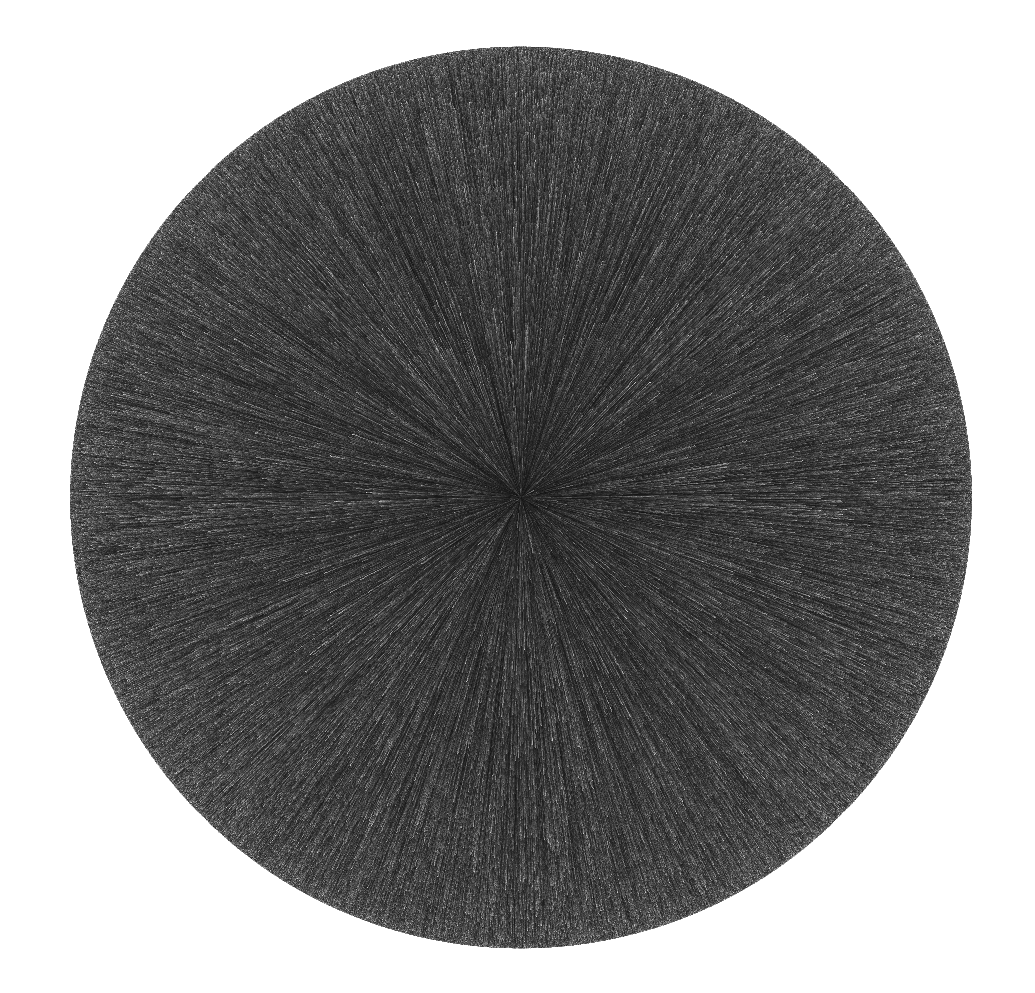
\includegraphics[width = 1.5 in]{3.png}
  \caption{
Where $D = 3$, as viewed from the side.
The field lines are isotropic, spherical.
}
\end{figure}
\begin{figure} 
\centering
\label{fig2}
  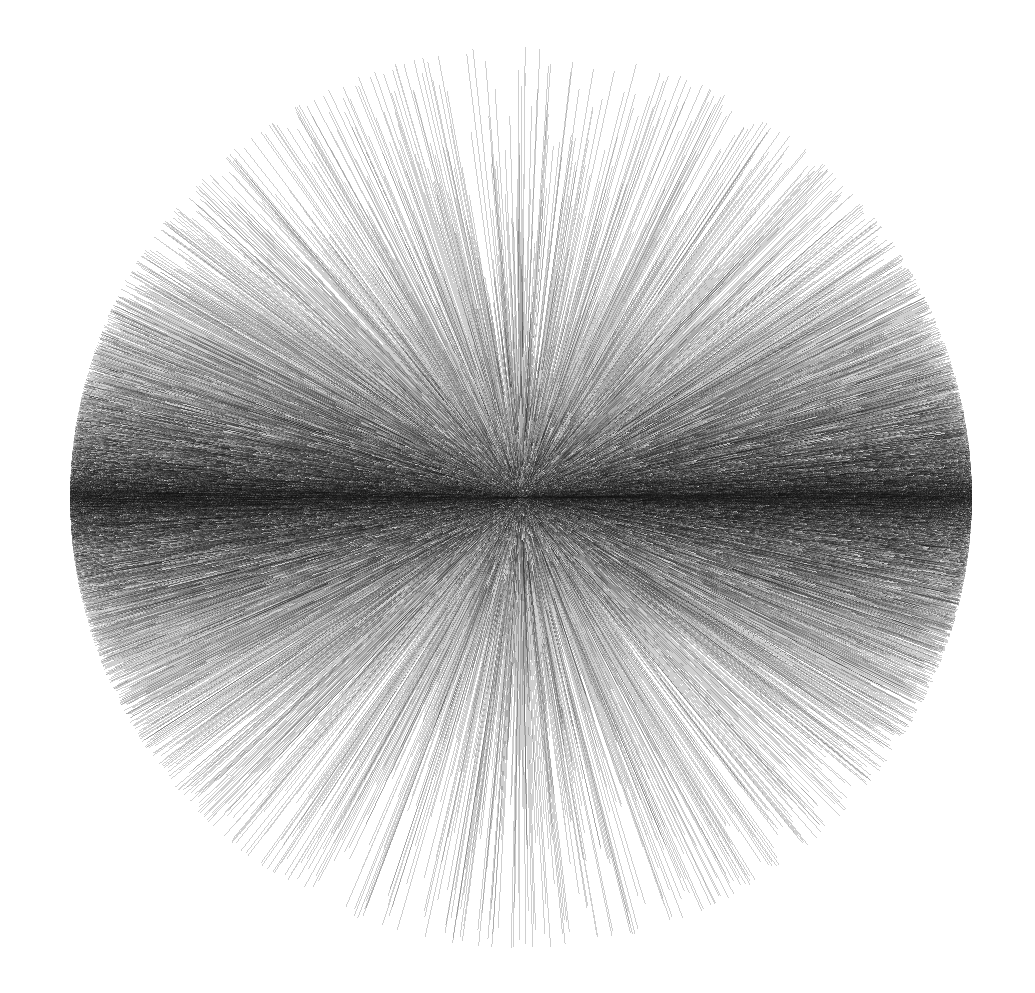
\includegraphics[width = 1.5 in]{2.1.png}
  \caption{
Where $D = 2.1$, as viewed from the side.
The field lines are increasingly anisotropic.
}
\end{figure}
\begin{figure} 
\centering
\label{fig3}
  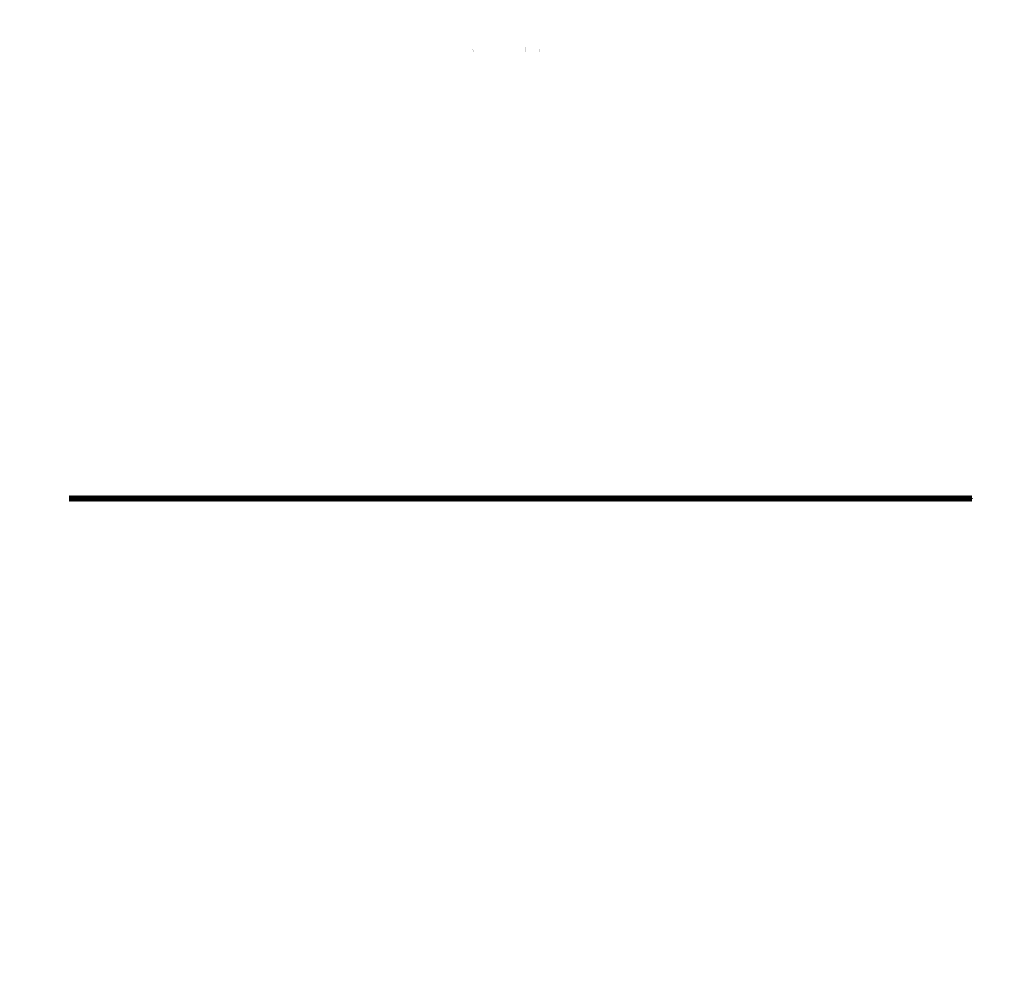
\includegraphics[width = 1.5 in]{2.001.png}
  \caption{
Where $D = 2$, as viewed from the side.
The field lines are anisotropic, disk-like.
}
\end{figure}





\begin{figure} 
\centering
\label{fig4}
  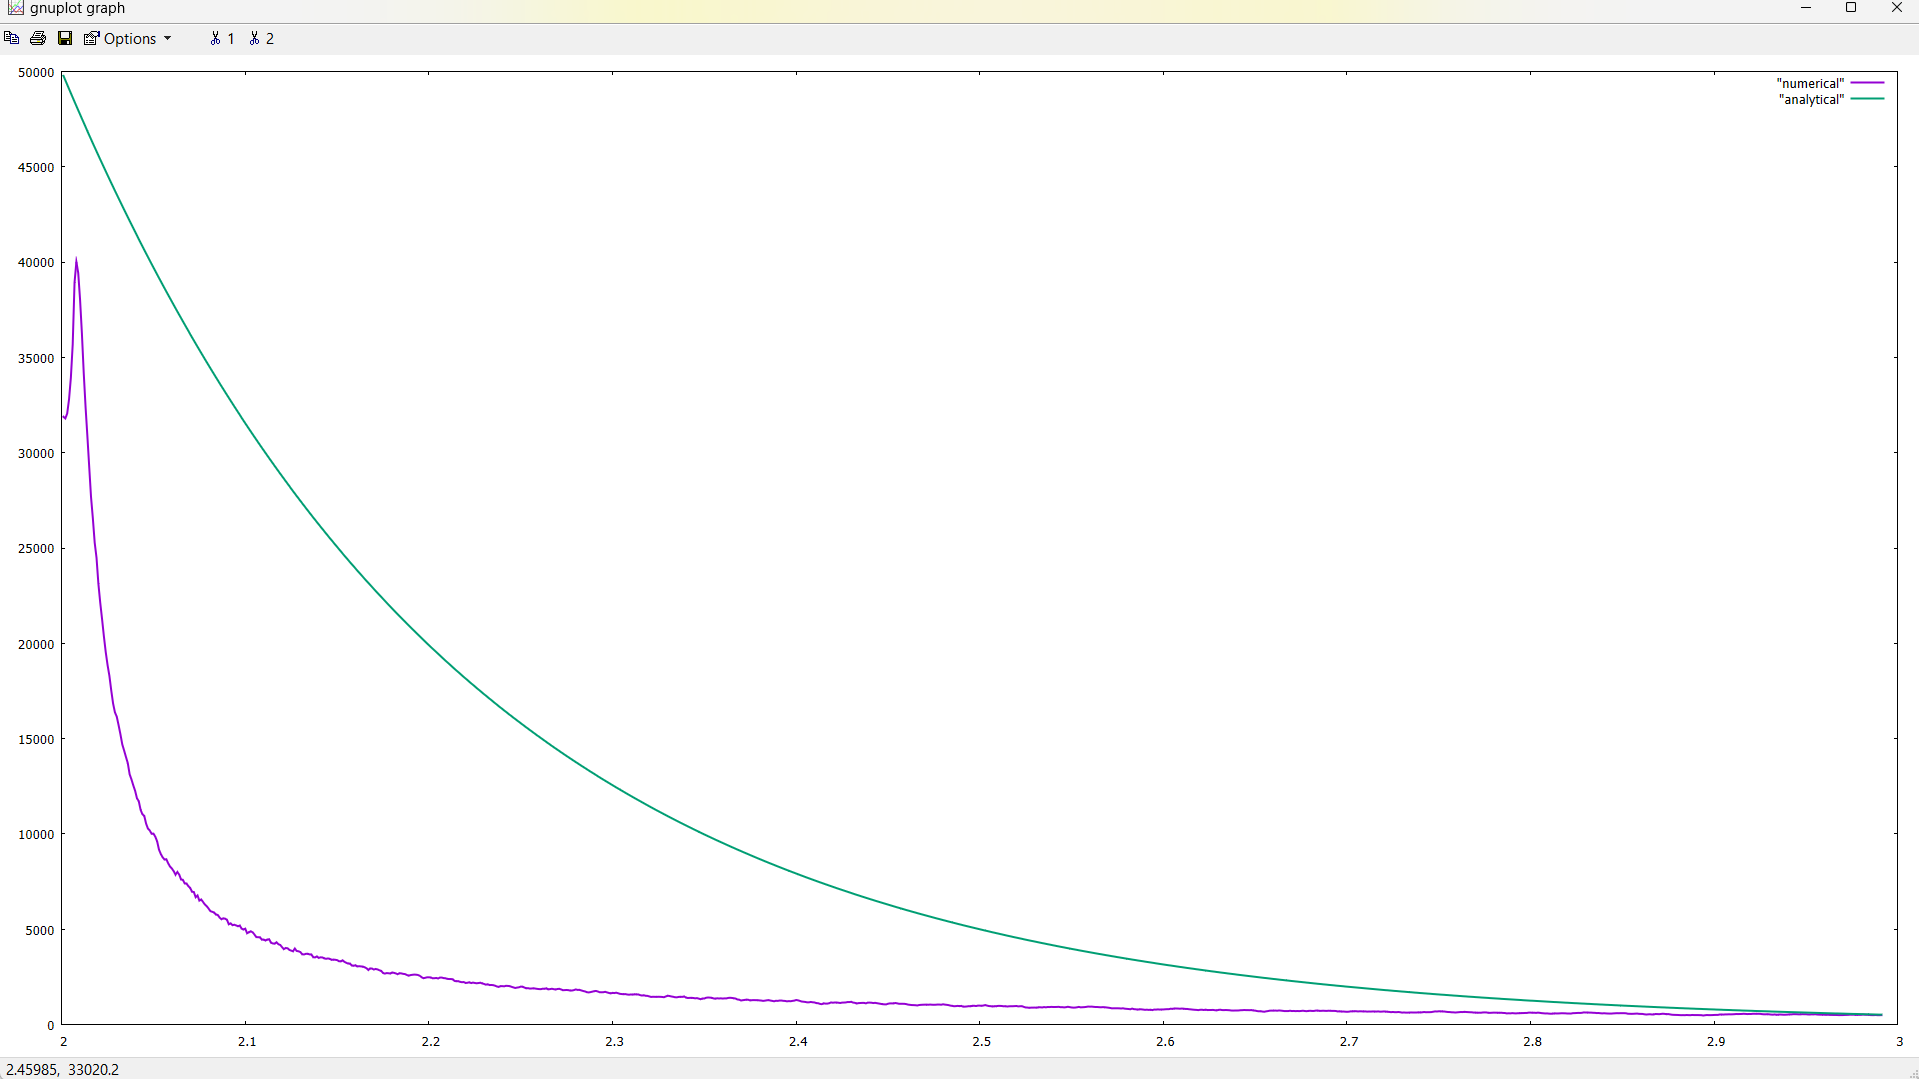
\includegraphics[width = 7 in]{numerical_versus_analytical.png}
  \caption{
Where $D = [2, 3]$, $R = 100$, $r = 1$, $n = $ 10e8, and $\epsilon = 1$.
The numerical plot (purple) is the gradient strength -- note that the plot is not monotonic.
For comparison, the analytical plot (green) is generated by the formula $y = n / (2 R^D)$.
}
\end{figure}


\begin{figure} 
\centering
\label{fig6}
  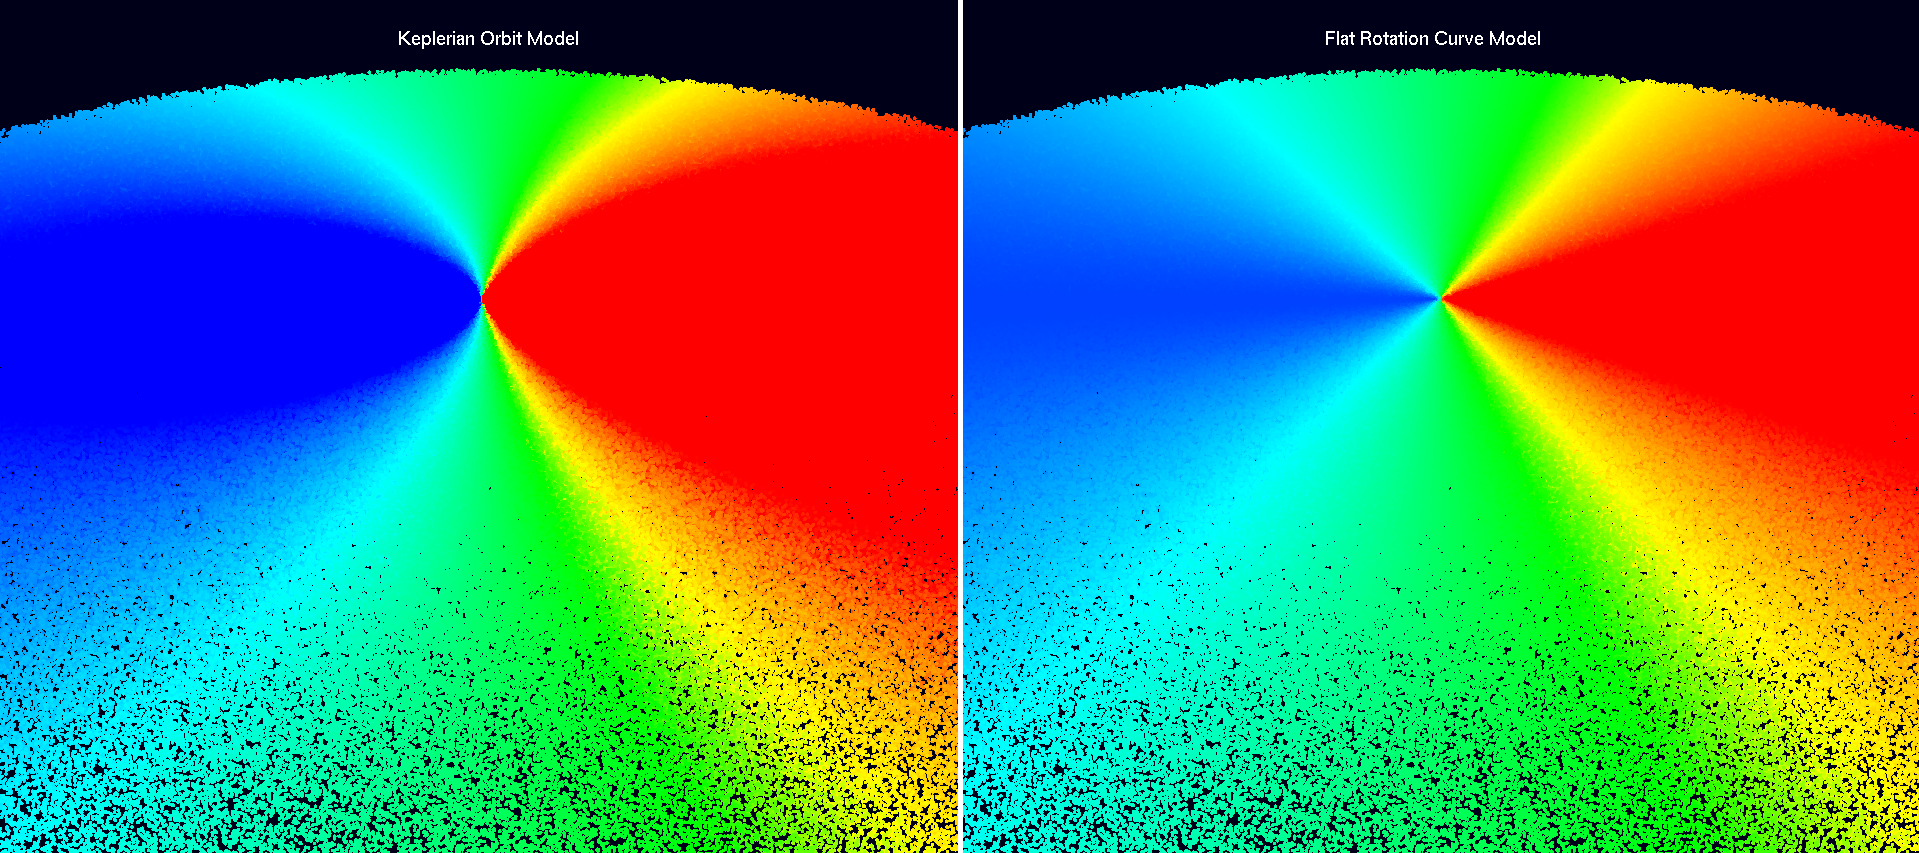
\includegraphics[width = 7 in]{doppler.png}
  \caption{
Visualization of the relativistic Doppler effect for 10e6 stars.
The Keplerian orbit is on the left, and the flat rotation curve orbit is on the right.
The redshift of the wavelength indicates stars moving away from the camera, and blueshift of the wavelength indicates stars moving toward the camera.
Thus, the stars in the galaxy are orbiting counterclockwise.
On the left, the wavelength is dependent on angle and distance from the galactic centre.
On the right, the wavelength is dependent only on angle, which means that there is a constant orbit speed that is independent of the distance from the galactic centre.
This is exactly what Vera Rubin discovered in the disks of the galaxies that she observed, and so dark matter was posited.
The Keplerian model (e.g. a protoplanetary disk) is full of isotropic pressure.
The flat rotation curve model (e.g. a galaxy) is pressure-free -- there is practically no interstellar pressure.
}
\end{figure}












\end{document}









